% Chapter Template

\chapter{Disseny} % Main chapter title

\label{Chapter6} % Change X to a consecutive number; for referencing this chapter elsewhere, use \ref{ChapterX}

Després d'haver mencionat, de forma molt específica, com és l'aplicació tant en requisits com en objectius, hem de veure com està construïda internament, és a dir, quin tipus d'arquitectura tècnica segueix, quin disseny de base de dades s'ha establert, com s'ha dissenyat el software implementat i amb quins patrons s'ha construït i finalment com s'ha definit la interfície de l'usuari.

%----------------------------------------------------------------------------------------
% SECTION 1
%----------------------------------------------------------------------------------------

\section{Arquitectura del sistema}

Després d'haver explicat quin és l'abast i quins objectius té \textit{Wisebite}, es va prendre la decisió que el projecte esdevingués a una plataforma mòbil per a dispositius Android. La justificació d'aquest fet ve dividida en dos punts, primer el fet que sigui un mòbil i no pas una aplicació web, per exemple, i l'altre pel fet que només s'hagi implementat per Android i no pas per cap altra sistema operatiu d'aquest tipus.
\\\\
En primera instància, el motiu principal pel qual \textit{Wisebite} ha estat implementat i dissenyat per dispositius mòbils és el dinamisme que aporten i del qual no disposen els dispositius de sobretaula. El món de la restauració és un sector de moviment continu, tant per part de l'empleat com per part del client. Un treballador d'un bar o restaurant es mourà de forma contínua per l'establiment i un client no sol acudir al mateix restaurant sempre. En conseqüència, el fet que \textit{Wisebite} estigui disponible en telèfons mòbils o bé tauletes permet als usuaris d'aquesta plataforma interactuar amb ella des de qualsevol lloc i de forma més còmode interactuant amb la pantalla tàctil que disposa el terminal.
\\\\
Per altra banda, \textit{Wisebite} s'ha especialitzat en sistemes operatius Android i no pas en algun altre per un seguit de factors que es comenten a continuació.
\\\\
En primer lloc és important recordar un dels tres factors pels quals sistemes d'aquest tipus no han acabat d'introduir-se dins el sector: el factor econòmic. En el mercat dels dispositius mòbils és vist i reconegut que els dispositius Android, donat el gran número de terminals en els quals opera, són de preu més reduït que pas els sistemes iOS, implementats per Apple. Així doncs, és important oferir hardware barat als establiments que implantin \textit{Wisebite} per així reduir l'impacte econòmic que els pot ocasionar.
\\\\
En segon lloc, per què només per Android i no pas també per iOS? És cert que existeix un seguit de \textit{frameworks} que et permet desenvolupar aplicacions mòbils híbrides, és a dir, per a tots els sistemes operatius mòbils.
\\\\
La problemàtica principal d'aquest tipus de desenvolupament és el fet de no poder utilitzar tots els avantatges que et permet un sistema operatiu natiu en concret. Per exemple, si analitzem les aplicacions mòbils natives d'Android, veiem que tot el \textit{backend} de l'aplicació pot ser escrit en Java, C++ o bé Kotlin i el \textit{frontend} amb llenguatge d'etiquetes com és XML. En canvi, si es realitzes amb un dels \textit{frameworks} que ofereix el mercat s'escriuria en HTML, CSS i JavaScript, com si es tractés d'una pàgina web. Són maneres d'implementar aplicacions molt diferents, i per molt que aquests \textit{frameworks} ho vulguin simular al màxim no ho acaben d'aconseguir del tot. Així doncs, donat que un dels objectius clau que té \textit{Wisebite} és destacar per la seva interfície és molt millor implementar en llenguatge natiu donats els avantatges que t'ofereix.
\\\\
Per tant, donada aquesta justificació, l'aplicació correrà en dispositius exclusivament Android a partir de l'\textit{API 21} o versió \textit{5.0 Lollipop}, és a dir, en un 88.6\%\cite{androidOsAnalytics} dels dispositius de la marca de Google.
\\\\
Aquesta aplicació es comunica amb una base de dades no relacional (NoSQL) anomenada \textit{Firebase}. En apartats posteriors dins d'aquest mateix capítol s'explicarà com s'ha implementat l'esquema de dades dins d'aquest gestor, però abans en aquest apartat és important conèixer el perquè de l'elecció de \textit{Firebase} com a base de dades per a \textit{Wisebite}.
\\\\
\textit{Firebase} va ser comprada per Google el maig del 2016, fet que aporta serietat, fiabilitat i robustesa com a base de dades, és a dir, pertany a una de les institucions més importants dins el sector de la informàtica, per no dir el que més. Tot i així, el factor més important i pel qual es va decidir utilitzar aquesta base de dades no relacional és que la comunicació es realitza en temps real. Aquest aspecte és realment important sabent quina és la temàtica de l'aplicació. Es considera molt important aquest fet, ja que l'actualització automàtica de les dades sense necessitat de refresc manual facilita moltíssim la feina d'un cambrer o d'un cuiner a l'hora d'interactuar amb la plataforma. Així doncs, per aquest fet es va decidir implantar la base de dades dins de \textit{Firebase}.
\\\\
Per últim, l'aplicació emmagatzemarà les dades temporals en un \textit{SQLite} que actuarà de memòria cau dins de \textit{Wisebite}. La justificació de l'ús d'aquesta tecnologia ve donat pel fet que Android la utilitza de forma predefinida en les seves aplicacions natives.
\\\\
Per clarificar més el concepte i veure quina és la interacció de l'usuari amb \textit{Android}, \textit{Firebase} i \textit{SQLite}, es mostra a continuació una gràfica de l'arquitectura tècnica que s'ha decidit utilitzar a \textit{Wisebite}.
\begin{figure}[H]
\centering
\includegraphics[scale=0.25]{Figures/technical_architecture.png}
\caption{Arquitectura tècnica del sistema}
\end{figure}

%----------------------------------------------------------------------------------------
%	SECTION 2
%----------------------------------------------------------------------------------------

\section{Disseny de la base de dades}

Com s'ha comentat en l'apartat anterior, la base de dades de \textit{Wisebite} serà \textit{Firebase}. Aquesta base de dades funciona amb una estructura en forma d'arbre basant-se en el format JSON\cite{json}.
\\\\
Existeix un node pare o arrel anomenat \textit{wisebite-f7a53} del qual pengen tots els nodes restants. Per a tal de dissenyar una bona base de dades NoSQL de tipus clau-valor, com es \textit{Firebase}, és necessari tenir en compte un seguit de conceptes per seguir les bones pràctiques que les mateixes guies del gestor recomanen:
\begin{itemize}
\item El fet d'accedir a un node, fa que hagi de descarregar tot l'arbre del qual penja aquest node (amb tots els seus respectius fills). Per tant, la solució és disgregar els elements. Cal tenir cura en relacionar els components o nodes de la base de dades per poder-los processar correctament. Un bon mètode seria associar els elements via el seu identificador i no pas tot l'element.
\item Per realitzar relacions entre, per exemple, un restaurant i els usuaris als quals hi treballen podríem pensar en afegir un node fill per a cada usuari del restaurant. Això és ineficient en cas de tenir restaurants amb un gran nombre d'usuaris en ells. En conseqüència, la solució seria utilitzar índexs. Per a cada restaurant s'hauria de tenir un llistat d'usuaris on es representen els usuaris pertanyents a ell.
\end{itemize}

\noindent Llavors, en definitiva, el missatge més important és que cal tenir en compte que encara que \textit{Firebase} tingui una estructura en forma d'arbre, no s'ha de construir  esquema de profunditat molt gran, sinó millor crear un arbre amb la major amplada possible. Això farà més eficient les consultes a la base de dades.
\\\\
Després d'haver estudiat i entès quines són les bones pràctiques d'una base de dades no relacional de tipus clau-valor, s'ha dissenyat de tal manera que pengen nou nodes del node arrel, on allà s'emmagatzemen totes les instàncies d'aquella entitat. Cadascuna d'elles serà identificada a partir d'un identificador aleatori. Cadascun d'aquest nodes representen les nou entitats que han estat explicades en capítols anteriors. A continuació es mostra l'estructura de la base de dades en format JSON.

\clearpage
\begin{lstlisting}[language=json,firstnumber=1]
"wisebite-f7a53" : {
   "dish" : {
      "-KlPZWq5d4cFO6NJ0nc4" : {
         "description" : "Classic",
         "id" : "-KlPZWq5d4cFO6NJ0nc4",
         "name" : "Paella",
         "price" : 12,
         "reviews" : {
            "-KlyJ20Nr3OpnA0JLqk5" : true,
            "-Km3Q9par9GavvZHt-4L" : true,
            "-KmNrn1Gxu66N6tc5u32" : true
         }
      },
      ...
   },
   "image" : {
      "-KlPTsD8xjazZ8KceJ6E" : {
         "description" : "Profile photo",
         "id" : "-KlPTsD8xjazZ8KceJ6E",
         "imageFile" : "https://lh5.googleuser..."
      },
      ...
   },
   "menu" : {
      "-KlPeMorCJsXKHh024Ui" : {
         "description" : "nu",
         "id" : "-KlPeMorCJsXKHh024Ui"
         "mainDishes" : {
            "-KlPeLzph1_Sz7UGcnMc" : true
         },
         "name" : "menu",
         "otherDishes" : {
            "-KlPeLzrWp_u0Fx3bNPW" : true
         },
         "price" : 0.5,
         "secondaryDishes" : {
            "-KlPeLzrWp_u0Fx3bNPV" : true
         }
      },
      ...
   },
   "openTime" : {
      "-KlPY8bUts4c9domVn5d" : {
         "endDate" : {
            "date" : 29,
            "day" : 1,
            "hours" : 22,
            "minutes" : 0,
            "month" : 11,
            "seconds" : 0,
            "time" : -180000000,
            "timezoneOffset" : 0,
            "year" : 69
         },
         "id" : "-KlPY8bUts4c9domVn5d",
         "startDate" : {
            "date" : 29,
            "day" : 1,
            "hours" : 8,
            "minutes" : 0,
            "month" : 11,
            "seconds" : 0,
            "time" : -230400000,
            "timezoneOffset" : 0,
            "year" : 69
         }
       },
       ...
    },
   "order" : {
      "-KlZianOlkFpEkNFoiF7" : {
         "date" : {
            "date" : 1,
            "day" : 4,
            "hours" : 19,
            "minutes" : 35,
            "month" : 5,
            "seconds" : 58,
            "time" : 1496338558814,
            "timezoneOffset" : -120,
            "year" : 117
         },
         "id" : "-KlZianOlkFpEkNFoiF7",
         "lastDate" : {
            "date" : 1,
            "day" : 4,
            "hours" : 20,
            "minutes" : 37,
            "month" : 5,
            "seconds" : 53,
            "time" : 1496342273505,
            "timezoneOffset" : -120,
            "year" : 117
         },
         "orderItems" : {
            "-KlZian7yy0XgIJaGrCV" : true,
            "-KlZianHOSo5hbzboxWl" : true,
            "-KlZianKOdNMI1r06jnh" : true,
            "-KlZianMs7fEFfK3JJw7" : true
         },
         "tableNumber" : 9
      },
      ...
   },
   "orderItem" : {
      "-KlYSoFkb_Z7WmMsvNEy" : {
         "delivered" : false,
         "dishId" : "-KlPeMorCJsXKHh024Uh",
         "id" : "-KlYSoFkb_Z7WmMsvNEy",
         "menuId" : null,
         "paid" : true,
         "ready" : false
      },
      ...
   },
   "restaurant" : {
      "-KlPZWqHH5fEgUoCrGG5" : {
         "description" : "De tota la vida, de poble.",
         "dishes" : {
            "-KlPZWq-xR39JAJBEitN" : true,
            "-KlPZWq1k46MlYinfido" : true,
            "-KlPZWq3w_Zwu63am50p" : true,
            "-KlPZWq4OshyHXIufnFO" : true,
            "-KlPZWq5d4cFO6NJ0nc4" : true
         },
         "externalOrders" : {
            "-Kldj4NCYd-3ZN9H93Mh" : true,
            "-Kldk-C2wrOFKZmrtOPB" : true,
            "-Kldt2L6ZRJouCK75rzP" : true,
            "-KlyIcuVp1Lx3U7235PN" : true,
            "-Km3Q3B4u_Sq65WCv0bq" : true,
            "-KmNqGKk-EURs6mBnQNz" : true
         },
         "id" : "-KlPZWqHH5fEgUoCrGG5",
         "location" : "Sant Celoni",
         "menus" : {
            "-KlPZWq7lAVXkCYqe-Z9" : true,
            "-KlPZWqDD_UhNEVauAtt" : true,
            "-KlPZWqF14E1wMPYIHT6" : true
         },
         "name" : "Cerveseria Ceres",
         "numberOfTables" : 30,
         "openTimes" : {
            "-KlPY8bUts4c9domVn5d" : true,
            "-KlPY8bnpSPVrvXvEL6F" : true,
            "-KlPY8brvVHqL0KXCfEi" : true,
            "-KlPY8bz9HQijw46-WWE" : true,
            "-KlPY8c2YzO4D7yZ99zU" : true
         },
         "phone" : 666544283,
         "reviews" : {
            "-KlyJ20VJ77rNt1Yfg2y" : true,
            "-Km3Q9pddyCuqWYlCz-C" : true,
            "-KmNrn1L9CSgClEUHv_I" : true
         },
         "users" : {
            "alsumo95@gmail@com" : true
         },
         "website" : "ceres.com"
       },
       ...
    },
   "review" : {
      "-KltwNoh4fDoG7tIWZYx" : {
         "comment" : "Rico!",
         "date" : {
            "date" : 8,
            "day" : 4,
            "hours" : 9,
            "minutes" : 21,
            "month" : 5,
            "seconds" : 12,
            "time" : 1496906472539,
            "timezoneOffset" : -120,
            "year" : 117
         },
         "id" : "-KltwNoh4fDoG7tIWZYx",
         "points" : 4,
         "userId" : "alsumo95@gmail@com"
      },
      ...
   },
   "user" : {
      "alripol95@gmail@com" : {
         "email" : "alripol95@gmail.com",
         "id" : "alripol95@gmail@com",
         "imageId" : "-Km0MSeurykImTbkBPEl",
         "lastName" : "Ripol",
         "myOrders" : {
            "-Km0RcztK3XoafmEAx4P" : true
         },
         "myRestaurants" : {
            "-Km0Nbs9ioiglQBNVNvv" : true
         },
         "name" : "Albert",
         "ordersToReview" : {
            "-Km0RcztK3XoafmEAx4P" : true
         }
      },
      ...
   }
}
\end{lstlisting}

%----------------------------------------------------------------------------------------
%	SECTION 3
%----------------------------------------------------------------------------------------

\section{Disseny de software}

Durant el transcurs de la carrera, i en especial durant l'especialitat d'Enginyeria del Software, s'ha emfatitzat molt en el concepte que programar bé no és simplement que funcioni el programa implementat, sinó que segueixi uns patrons específics que et permeti tenir un codi fàcil d'entendre i re-usable, ja que al cap i a la fi el codi es llegeix més cops dels que s'escriu.
\\\\
És per això que en la implementació del projecte de \textit{Wisebite} s'ha seguit un conjunt de patrons de disseny de software anomenats patró repositori, patró servei, patró factoria i el més conegut anomenat MVC (Model-Vista-Controlador).

\subsection{Patrons de disseny}

S'ha utilitzat, com s'ha comentat anteriorment, quatre patrons de disseny durant la implementació de \textit{Wisebite}.

\begin{itemize}
\item \textbf{Patró repositori}: utilitzat per evitar l'accés directe a les dades, és a dir, des de la vista o més concretament en Android, des de l'\textit{Activity}. En aquest cas es permet desacoblar al màxim l'accés a \textit{Firebase}. Tota classe que serà traduïda en un objecte persistent en \textit{Firebase}, seguint el model de la base de dades mostrat al capítol anterior, ha d'implementar una interfície \textit{Entity} definida (apèndix \ref{Entity}), i definirem una interfície \textit{Repository} (apèndix \ref{Repository}) parametritzada, sobre la qual caldrà implementar una classe \textit{RepositoryXXXX} (apèndix \ref{RepositoryXXXX}) que la implementi (on XXXX defineix l'objecte que emmagatzema el repositori), que seran instanciades i utilitzades amb els seus mètodes ja definits per accedir a \textit{Firebase}. Aquesta classe \textit{RepositoriXXXX} hereta d'una altre anomenada \textit{FirebaseRepository} (apèndix \ref{FirebaseRepository}) per així afegir una capa més d'abstracció.

\item \textbf{Patró servei / injecció de dependència}: utilitzat per crear una capa d'abstracció sobre els dipòsits prèviament esmentats. En aquestes noves classes, les quals hereten d'una interfície anomenada \textit{Service} (apèndix \ref{Service}), ens permet executar la lògica del programa, sense necessitat d'accedir directament als repositoris. Aquests serveis contenen una instància única del repositori. Gràcies a la injecció de dependència podem realitzar tests de la lògica del programa sense haver de fer servir la base de dades real mitjançant \textit{mocking} dels repositoris. Malauradament, donat al factor temporal i que especificarem en capítols posteriors, no s'ha posat a la pràctica la utilitat dels tests. Tot i així, el codi del programa està ben preparat per poder afegir tests fàcilment.

\item \textbf{Patró factoria}: utilitzat per a la crida de serveis amb la creació d'un singleton anomenat \textit{ServiceFactory} (apèndix \ref{ServiceFactory}). Permet abstreure la funcionalitat de creació del servei, permetent així evitar la creació repetitiva del servei a cada ús que se li dóna, fet que comportaria tenir moltes instàncies del mateix objecte repartides per l'execució de l'aplicació. Separa la instanciació del servei del seu ús. Permet que es faci injecció de dependències sense haver de saber l'estructura d'aquesta.

\item \textbf{MVC}: utilitzat per organitzar l'estructura de l'aplicació. En el cas de \textit{Wisebite} en tractar-se d'Android les vistes són les activities. D'altra banda els controladors s'han anomenat serveis.
\end{itemize}

%----------------------------------------------------------------------------------------
%	SECTION 4
%----------------------------------------------------------------------------------------

\section{Disseny de la interfície}

Com es va comentar en capítols anteriors, concretament en l'estudi de mercat, actualment existeixen aplicacions que en qüestió de funcionalitats s'assemblen o s'acosten al que busca \textit{Wisebite}, però la gran majoria d'aquestes no han dedicat molt temps en l'estudi de la gestió de la interfície d'usuari. En canvi, en aquest projecte s'ha dedicat més del temps mínim requerit per construir una interfície el millor possible per l'usuari.
\\\\
El primer factor que es va tenir en compte va ser l'ús de les directrius que marca el \textit{Material Design}, un estil de disseny d'interfícies que va néixer amb l'API 21 o versió 5.0 d'Android. Amb l'aparició d'aquest estil s'ha buscat en tot moment facilitar l'ús de les aplicacions a les persones que els hi costa més utilitzar aplicacions per a smartphones. Interfícies molt més intuïtives, de colors i formes característiques, amb més dinamisme en la navegació per la plataforma i, sobretot, un patró de disseny estable en tots els dispositius del mercat.
\\\\
\textit{Wisebite} ha decidit seguir aquest model, ja que és molt important no canviar molt la interfície a la qual està acostumat l'usuari amb altres aplicacions. Per aquest motiu doncs s'ha decidit seguir els dissenys pre-establerts que facilita les guies de \textit{Material Design}.
\\\\
Durant la navegació de l'aplicació s'ha buscat tenir transicions entre vistes per aplicar-li un extra de dinamisme en l'experiència de l'usuari. Es manté en tot moment a l'usuari assabentat de quin és l'estat de l'aplicació per així adquirir un grau més alt d'atenció. S'ha buscat que les vistes fossin el més intuïtives possibles, i s'ha decidit utilitzar una paleta de colors neutre amb l'ús del gris, negre i blanc per no ser massa arriscats en el joc de colors i buscar quelcom no massa lluny de la normalitat.
\\\\
Per aconseguir un producte el més pròxim a l'usuari real s'ha realitzat un seguit d'iteracions que han estat provades per usuaris externs al sistema. Se'ls hi mostrava una versió de l'aplicació, la qual la provaven sense cap tipus de guia prèvia ni aprenentatge i s'estudiaven quins eren els seus moviments naturals a l'hora d'interactuar amb la plataforma. A més a més, s'escoltava la opinió dels usuaris respecte als aspectes que ells i elles millorarien. Tot i així, la metodologia d'iteracions serà explicada amb més detall en capítols posteriors.
\\\\
Un cop explicat el concepte amb el qual s'ha treballat de base, a continuació es mostren vuit captures de pantalla de la plataforma per així poder visualitzar l'estat del producte final, després d'haver seguit les directrius comentades anteriorment.

\begin{figure}[!h]
\centering
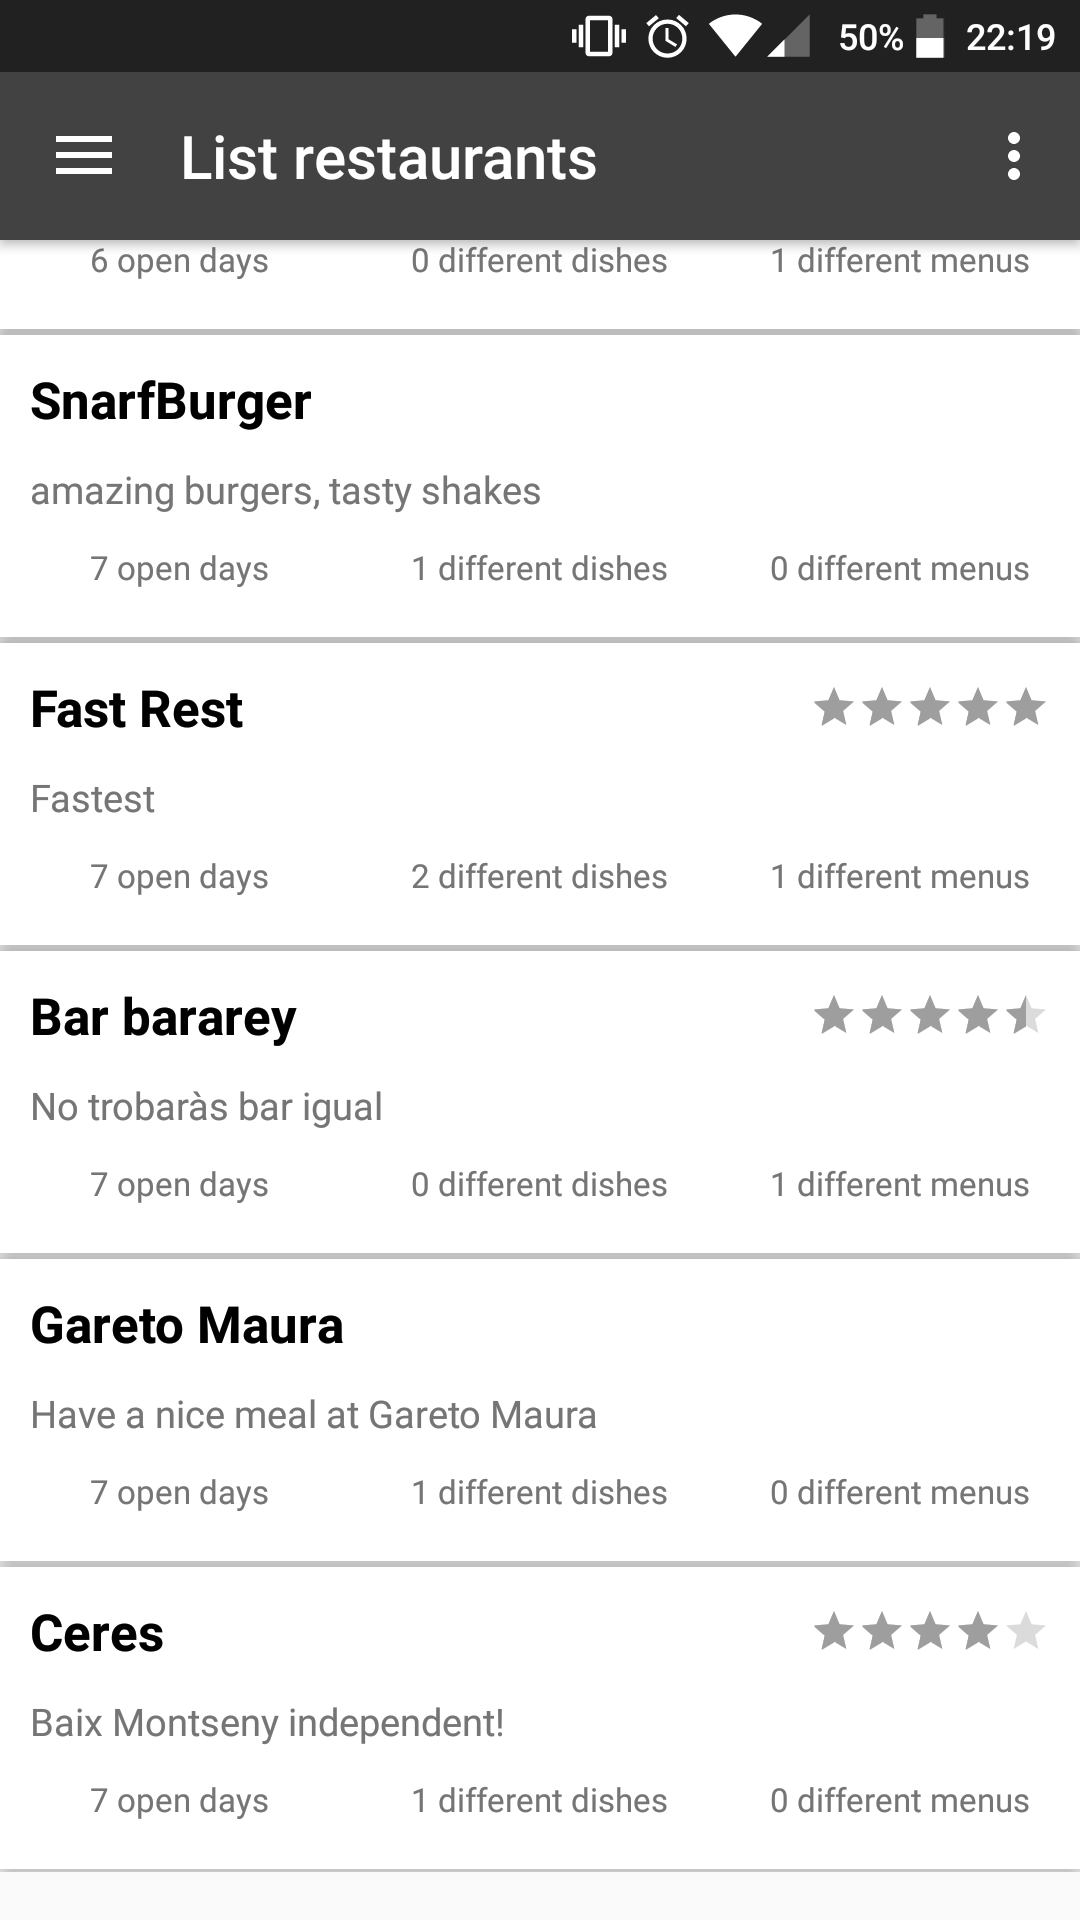
\includegraphics[scale=0.15]{Figures/wisebite_screenshot_1.png}
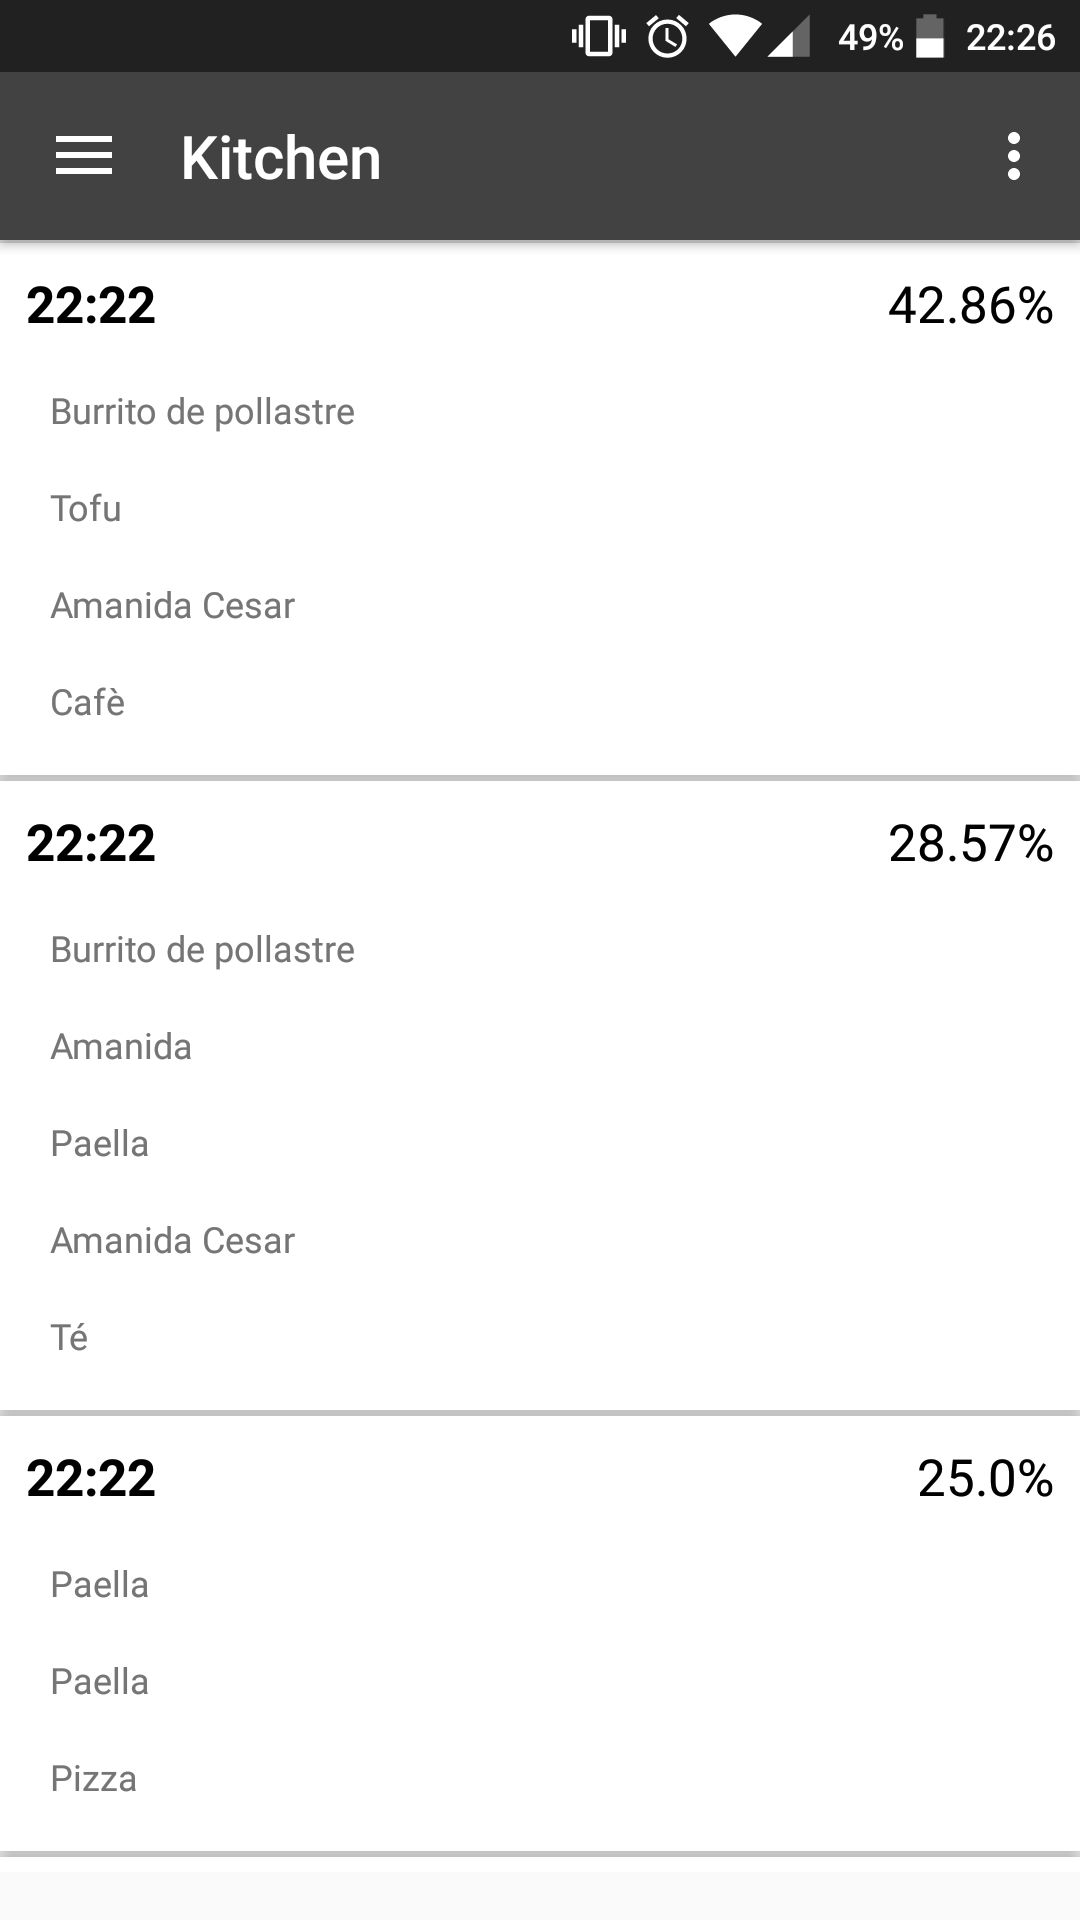
\includegraphics[scale=0.15]{Figures/wisebite_screenshot_2.png}
\caption{Captures de pantalla de Wisebite: llistat de restaurants i mode cuina}
\end{figure}

\begin{figure}[!h]
\centering
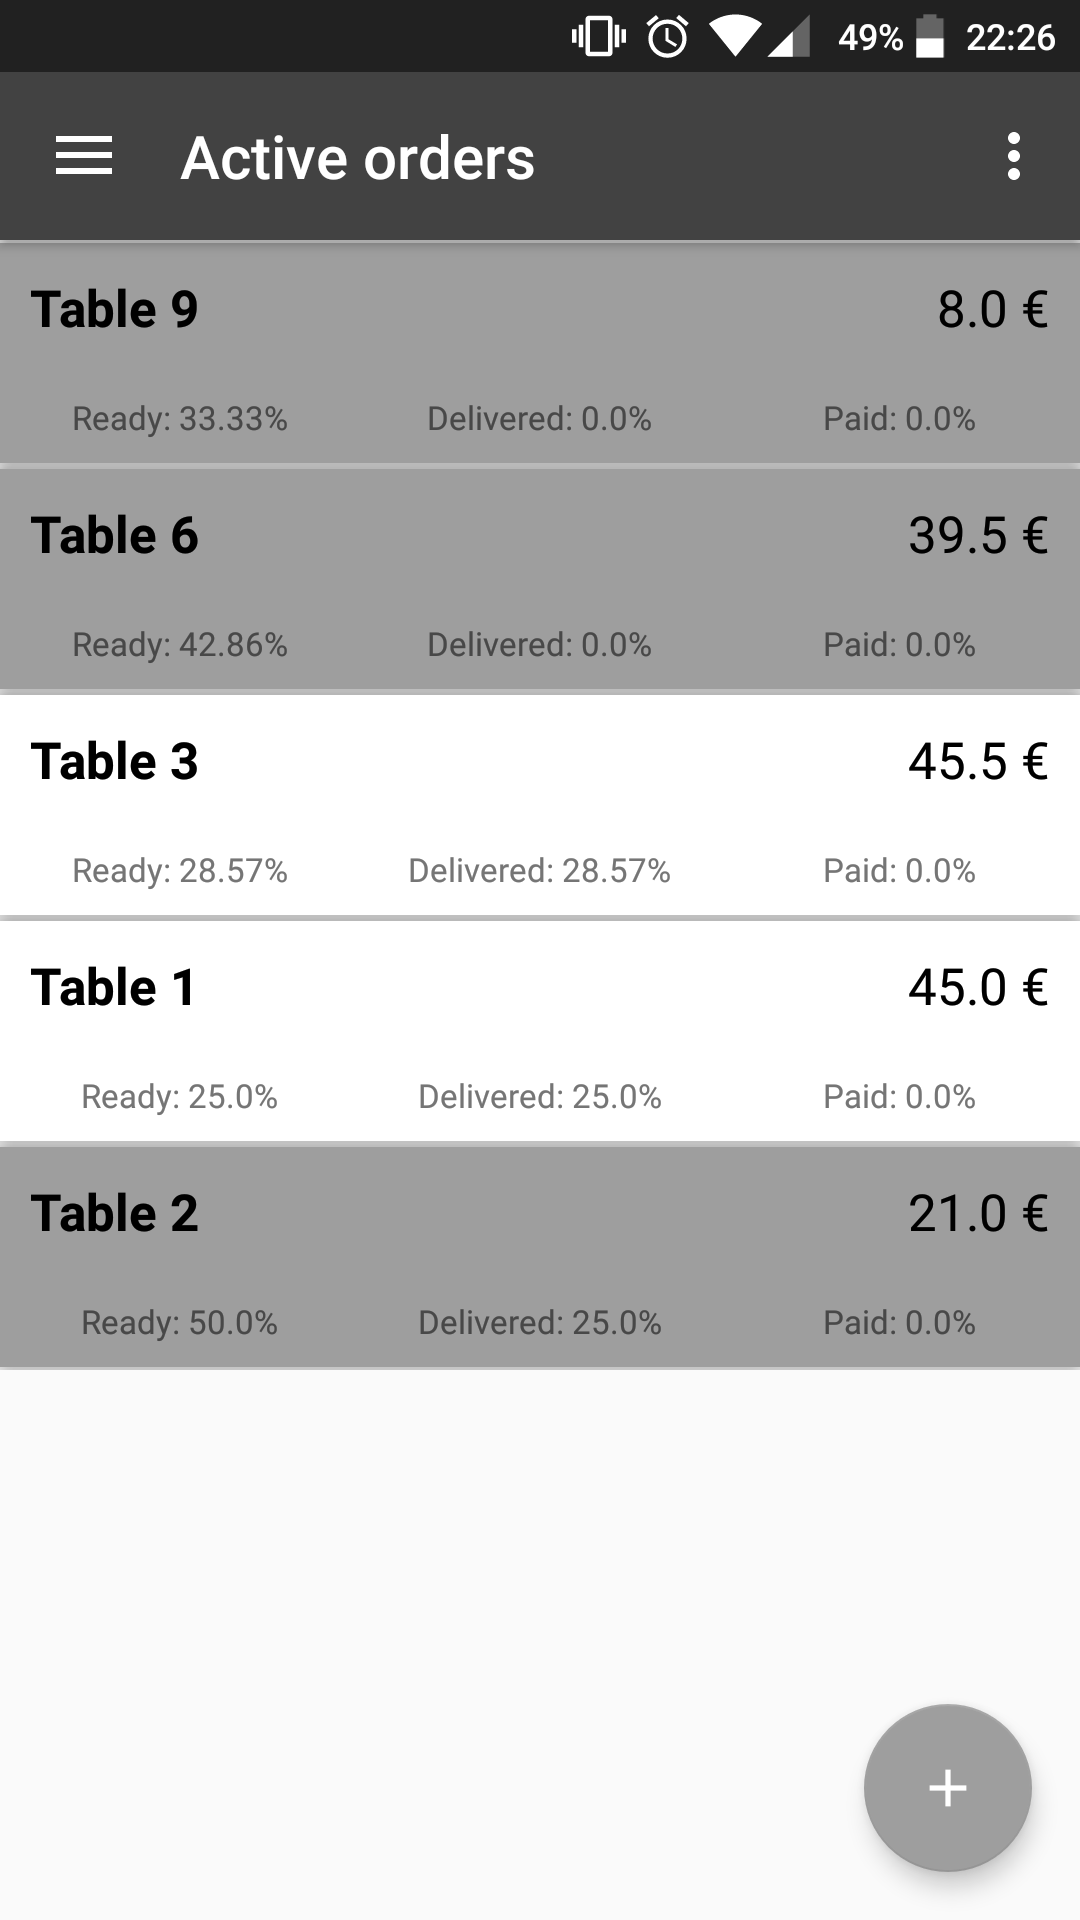
\includegraphics[scale=0.15]{Figures/wisebite_screenshot_3.png}
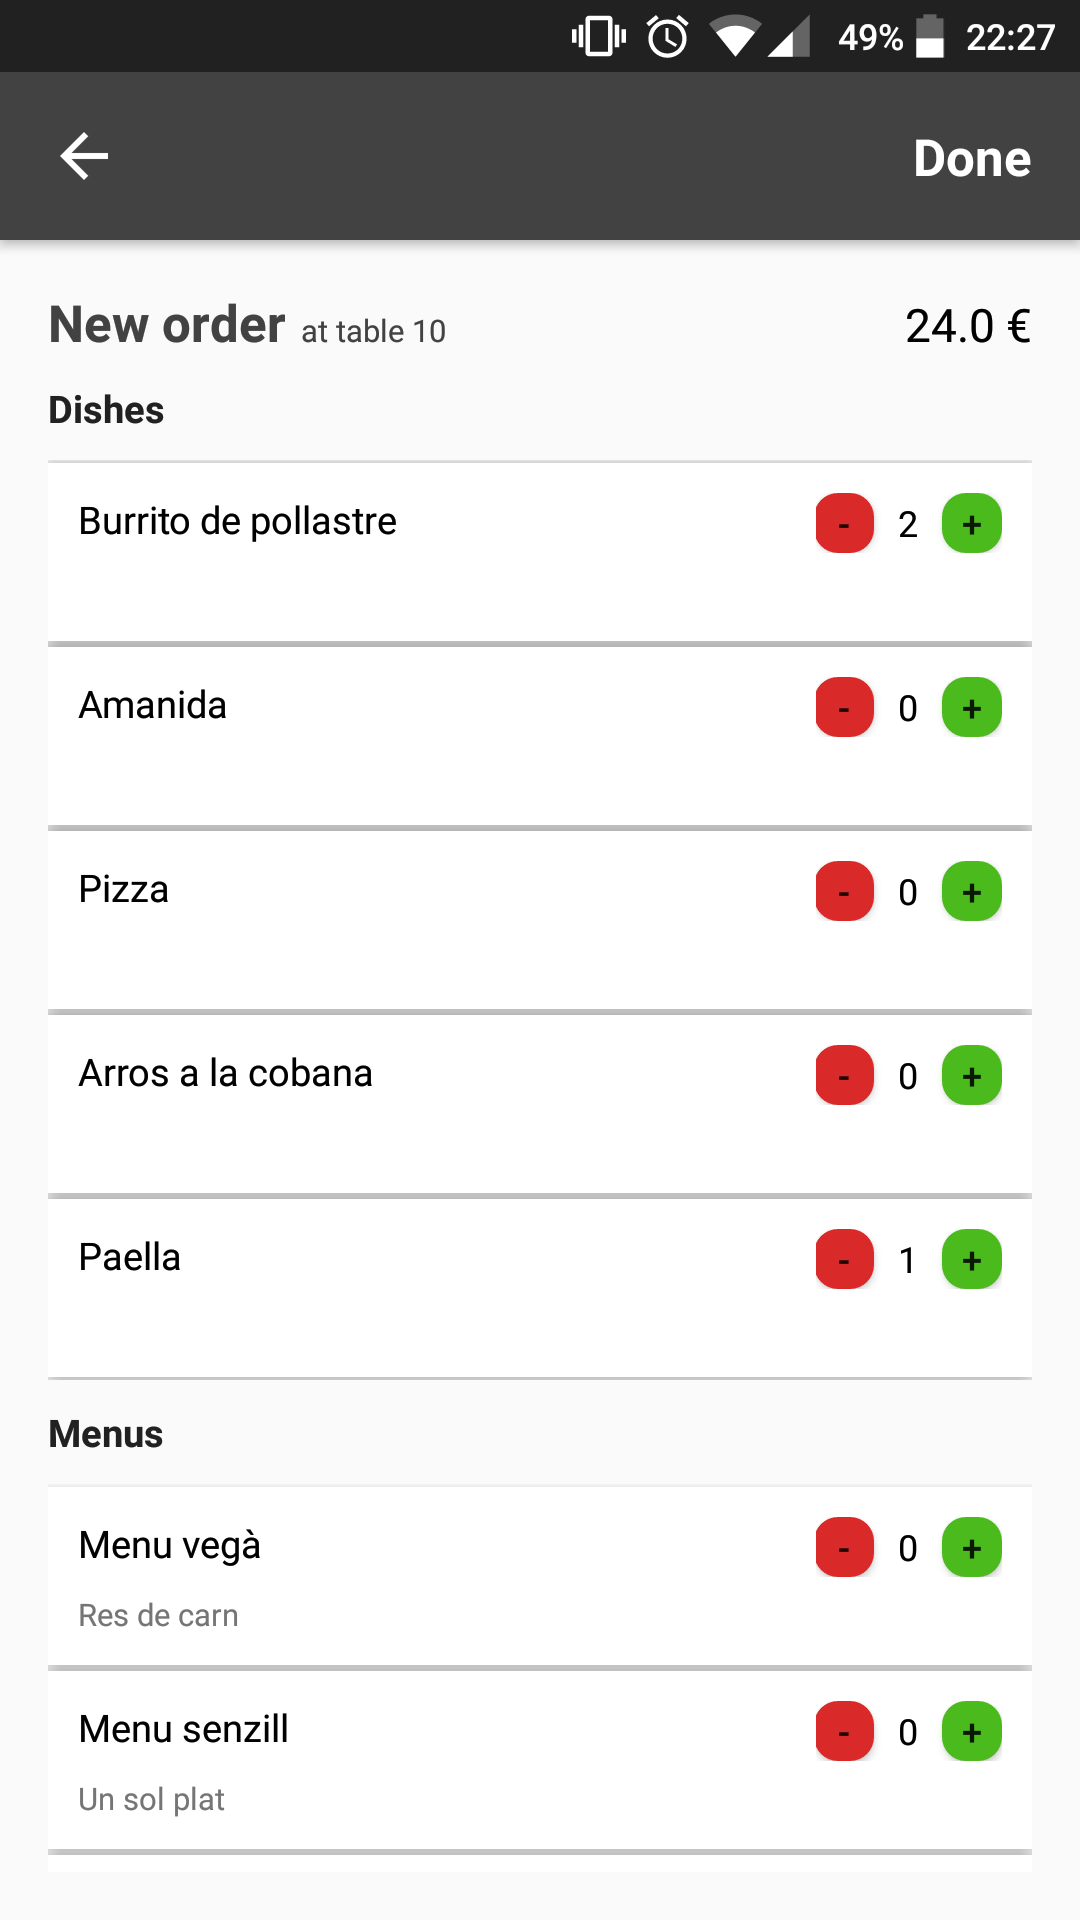
\includegraphics[scale=0.15]{Figures/wisebite_screenshot_4.png}
\caption{Captures de pantalla de Wisebite: llistat de comandes actives i consulta de comanda}
\end{figure}

\begin{figure}[!h]
\centering
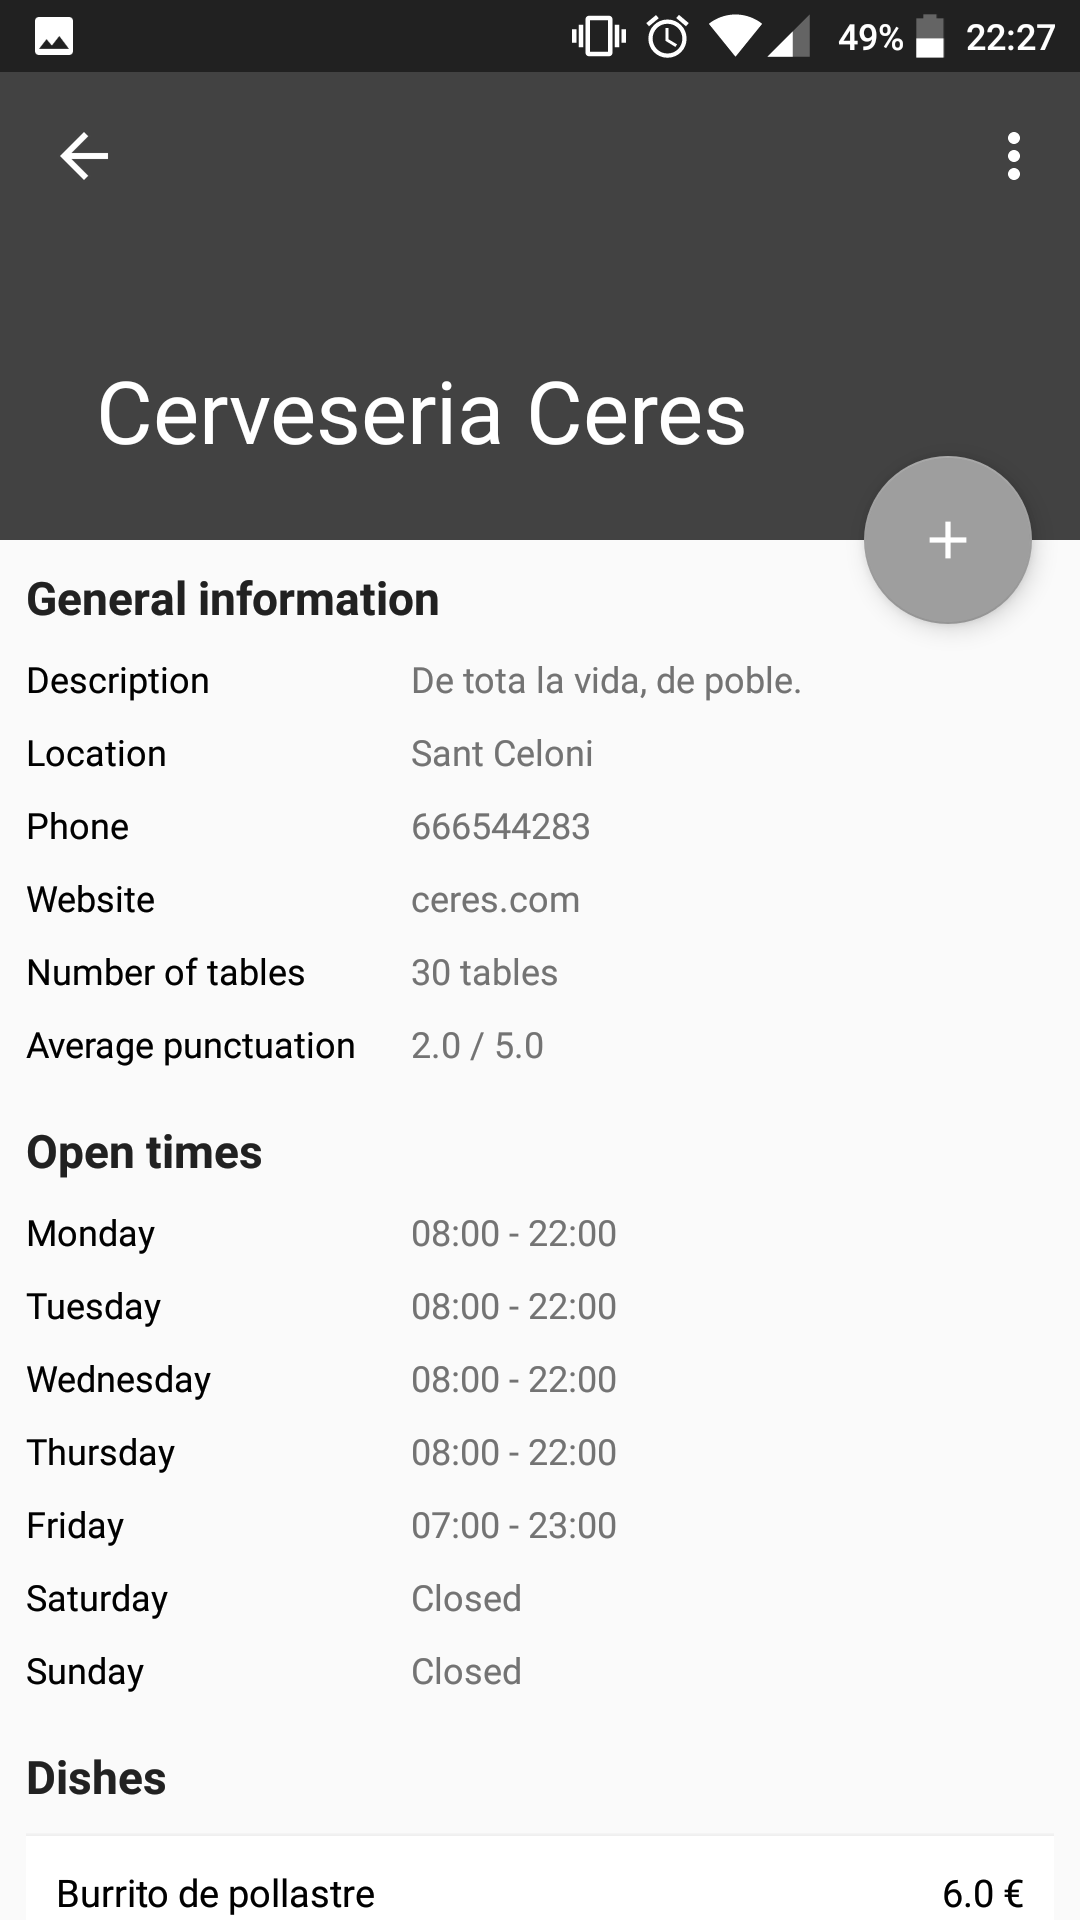
\includegraphics[scale=0.15]{Figures/wisebite_screenshot_5.png}
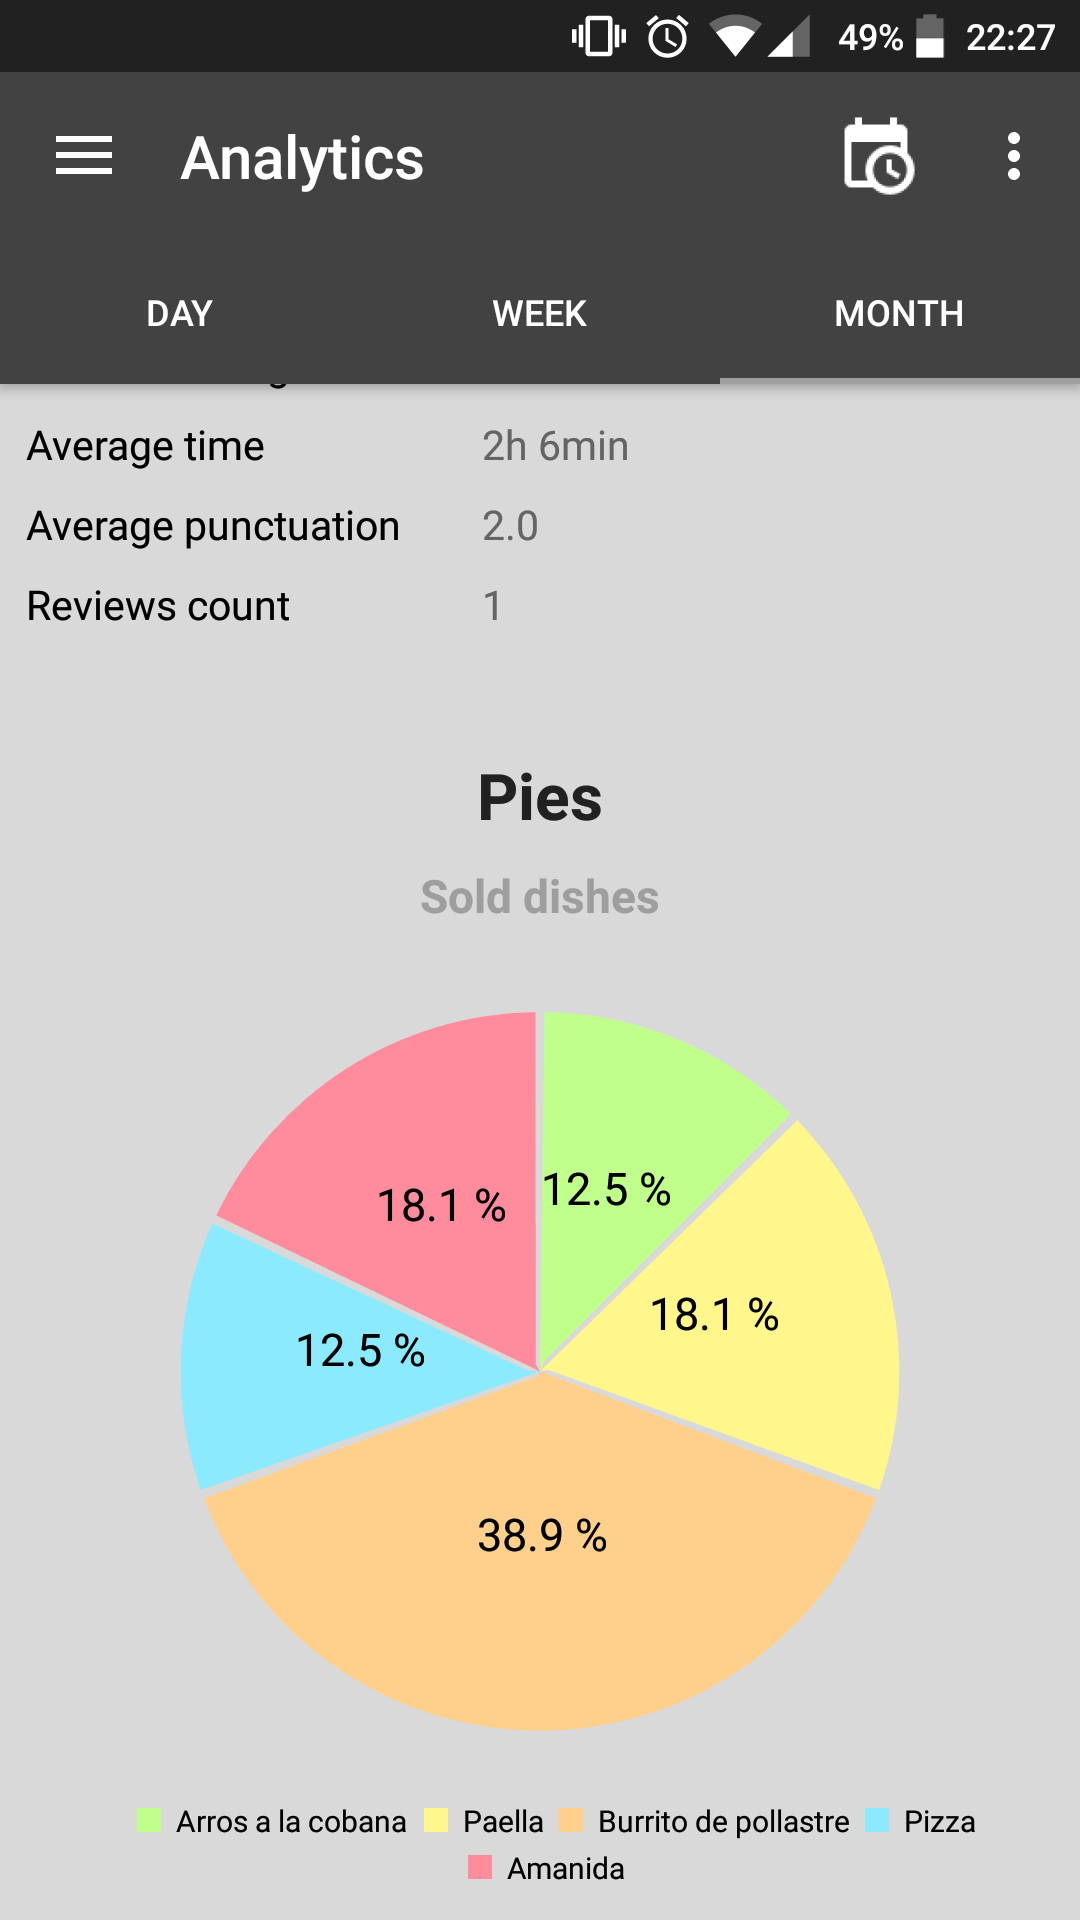
\includegraphics[scale=0.15]{Figures/wisebite_screenshot_6.png}
\caption{Captures de pantalla de Wisebite: consulta de restaurant i estadístiques}
\end{figure}

\begin{figure}[!h]
\centering
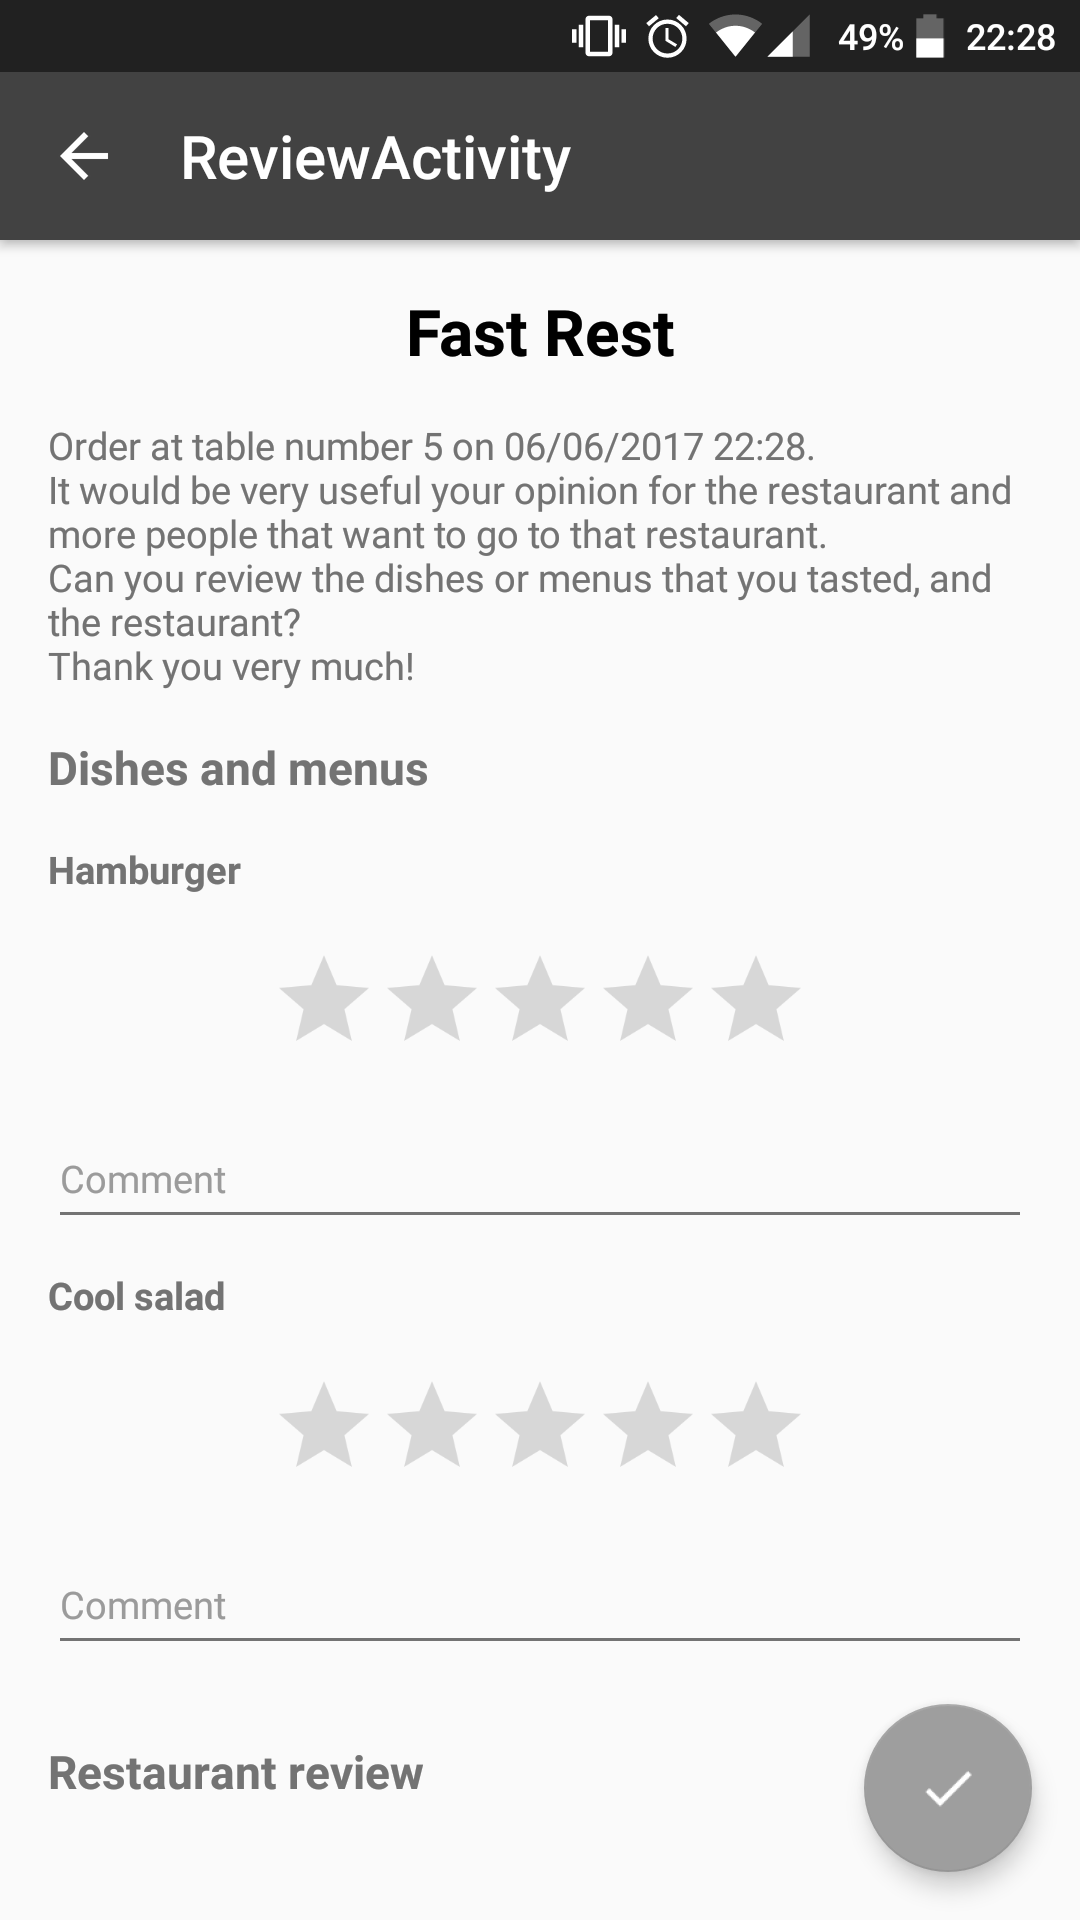
\includegraphics[scale=0.15]{Figures/wisebite_screenshot_7.png}
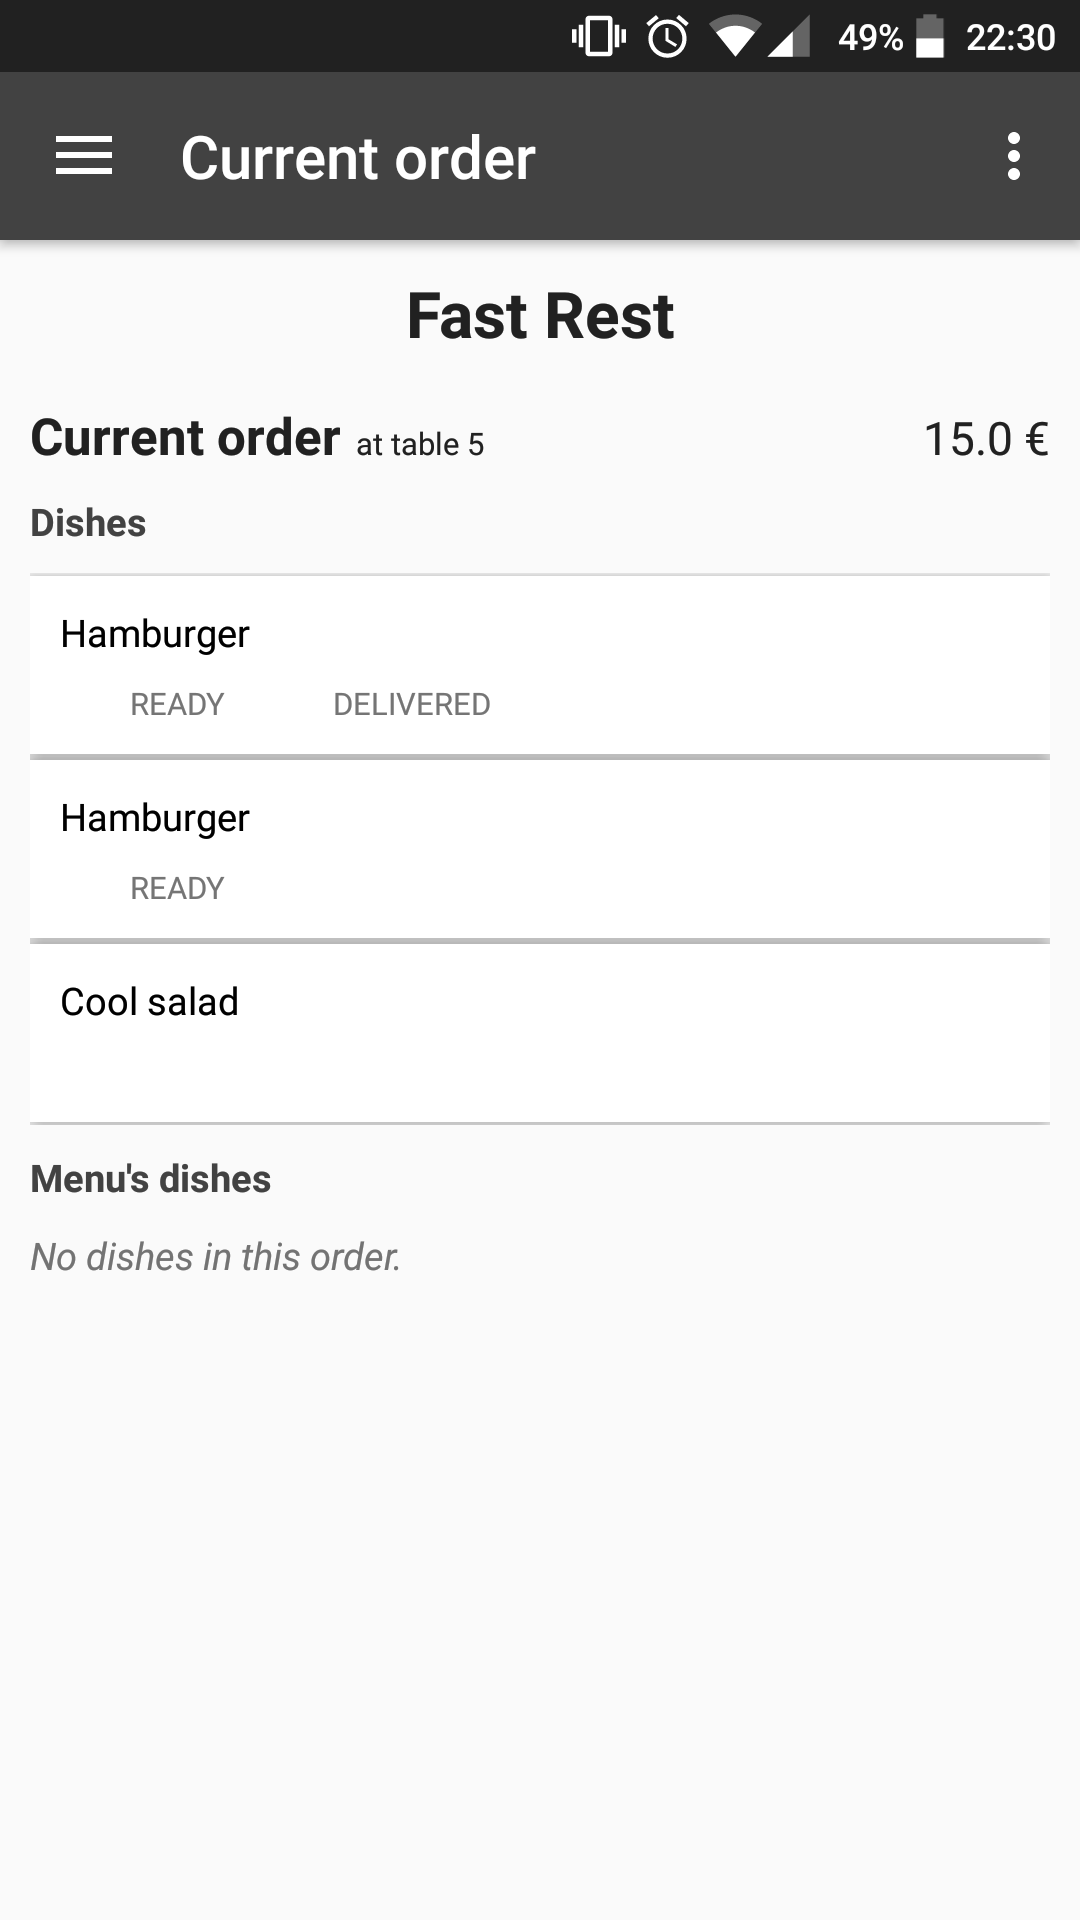
\includegraphics[scale=0.15]{Figures/wisebite_screenshot_8.png}
\caption{Captures de pantalla de Wisebite: valoració i comanda actual}
\end{figure}